%%%%%%%%%%%%%%%%%%%%%%%%%%%%%%%%%%%%%%%%%%%%%%%%%%%
%% LaTeX book template                           %%
%% Author:  Amber Jain (http://amberj.devio.us/) %%
%% License: ISC license                          %%
%%%%%%%%%%%%%%%%%%%%%%%%%%%%%%%%%%%%%%%%%%%%%%%%%%%

\documentclass[a4paper,11pt]{book}
\usepackage[T1]{fontenc}
\usepackage[utf8]{inputenc}
\usepackage{lmodern}
%%%%%%%%%%%%%%%%%%%%%%%%%%%%%%%%%%%%%%%%%%%%%%%%%%%%%%%%%
% Source: http://en.wikibooks.org/wiki/LaTeX/Hyperlinks %
%%%%%%%%%%%%%%%%%%%%%%%%%%%%%%%%%%%%%%%%%%%%%%%%%%%%%%%%%
\usepackage{hyperref}
\usepackage{graphicx}
\usepackage[english]{babel}
\usepackage[a4paper,top=2cm,bottom=2cm,left=2cm,right=2cm]{geometry}
\usepackage{lscape}
\usepackage{caption}
\usepackage{amsmath}
\usepackage{listingsutf8}
\usepackage{listings}
\usepackage{float}
\usepackage{amsmath}
\usepackage{subfig}
\usepackage{xcolor}
\usepackage{textcomp}
\usepackage{wrapfig}
\usepackage{rotating}
\usepackage{epstopdf}
\usepackage{commath}
\usepackage{systeme}
\usepackage{mathtools}
\usepackage{siunitx}
\definecolor{codegreen}{rgb}{0,0.6,0}
\definecolor{codegray}{rgb}{0.5,0.5,0.5}
\definecolor{codepurple}{rgb}{0.58,0,0.82}
\definecolor{backcolour}{rgb}{0.95,0.95,0.92}

\lstdefinestyle{mystyle}{
	backgroundcolor=\color{backcolour},   
	commentstyle=\color{codegreen},
	keywordstyle=\color{magenta},
	numberstyle=\tiny\color{codegray},
	stringstyle=\color{codepurple},
	basicstyle=\ttfamily\footnotesize,
	language = Matlab,
	frameround=fttt,
	frame = trBL,
	firstnumber = last,
	breakatwhitespace=false,         
	breaklines=true,                 
	captionpos=b,                    
	keepspaces=true,                 
	numbers=left,                    
	numbersep=5pt,                  
	showspaces=false,                
	showstringspaces=false,
	showtabs=false,                  
	tabsize=2
}

\lstset{style=mystyle}

\captionsetup{tableposition=top,figureposition=bottom,font=small}
%%%%%%%%%%%%%%%%%%%%%%%%%%%%%%%%%%%%%%%%%%%%%%%%%%%%%%%%%%%%%%%%%%%%%%%%%%%%%%%%
% 'dedication' environment: To add a dedication paragraph at the start of book %
% Source: http://www.tug.org/pipermail/texhax/2010-June/015184.html            %
%%%%%%%%%%%%%%%%%%%%%%%%%%%%%%%%%%%%%%%%%%%%%%%%%%%%%%%%%%%%%%%%%%%%%%%%%%%%%%%%
\newenvironment{dedication}
{
   \cleardoublepage
   \thispagestyle{empty}
   \vspace*{\stretch{1}}
   \hfill\begin{minipage}[t]{0.66\textwidth}
   \raggedright
}
{
   \end{minipage}
   \vspace*{\stretch{3}}
   \clearpage
}

%%%%%%%%%%%%%%%%%%%%%%%%%%%%%%%%%%%%%%%%%%%%%%%%
% Chapter quote at the start of chapter        %
% Source: http://tex.stackexchange.com/a/53380 %
%%%%%%%%%%%%%%%%%%%%%%%%%%%%%%%%%%%%%%%%%%%%%%%%
\makeatletter
\renewcommand{\@chapapp}{}% Not necessary...
\newenvironment{chapquote}[2][2em]
  {\setlength{\@tempdima}{#1}%
   \def\chapquote@author{#2}%
   \parshape 1 \@tempdima \dimexpr\textwidth-2\@tempdima\relax%
   \itshape}
  {\par\normalfont\hfill--\ \chapquote@author\hspace*{\@tempdima}\par\bigskip}
\makeatother

%%%%%%%%%%%%%%%%%%%%%%%%%%%%%%%%%%%%%%%%%%%%%%%%%%%
% First page of book which contains 'stuff' like: %
%  - Book title, subtitle                         %
%  - Book author name                             %
%%%%%%%%%%%%%%%%%%%%%%%%%%%%%%%%%%%%%%%%%%%%%%%%%%%

% Book's title and subtitle
\title{
	
\includegraphics[width=0.7\textwidth]{Immagini/UniBg.png}
	\\ \Huge \textbf{VAB - Veicolo auto bilanciato} \\ \huge \textit{\textbf{Relazione di progetto}} \\ \bigskip \huge Laboratorio di Sistemi Meccatronici II\\ Università degli Studi di Bergamo\\ \textit{Kilometro rosso} \\ \huge A.A. 2019/2020}
% Author
\author{\textsc{Calegari Andrea - 1041183}
		\\ \textsc{Piffari Michele - 1040658}}

\begin{document}
	
	\frontmatter
	\maketitle
	%%%%%%%%%%%%%%%%%%%%%%%%%%%%%%%%%%%%%%%%%%%%%%%%%%%%%%%%%%%%%%%%%%%%%%%%
	% Auto-generated table of contents, list of figures and list of tables %
	%%%%%%%%%%%%%%%%%%%%%%%%%%%%%%%%%%%%%%%%%%%%%%%%%%%%%%%%%%%%%%%%%%%%%%%%
	\tableofcontents
	\listoffigures
	
	
	\mainmatter
	\chapter{Introduzione}
	L'approccio seguito per la stesura del modello dinamico del veicolo autobilanciato ha da subito preso una via meno \textit{tradizionale} rispetto al classico metodo risolutivo: abbiamo infatti preferito, dato il nostro \textit{background} informatico, approcciare il problema direttamente in ambiente Matlab, sfruttando sin da subito le potenzialità di calcolo offerte dal software di \textit{Mathworks}.

Nello specifico, per la parte di stesura e definizione della dinamica, abbiamo inzialmente seguito una via risolutiva duale, portando avanti sia un'analisi letterale, sfruttando le potenzialità del \textbf{calcolo simbolico} messe a disposizione delle funzionalità di \textbf{live scripting}, sia uno studio numerico (considerando quindi le varie grandezze fisiche con i valori definiti delle specifiche di progetto).

In linea di massima lo sviluppo del progetto ha seguito un andamento a step graduali, cadenziati da incontri settimanali in cui poter confrontare e consolidare lo \textit{stato di avanzamento dei lavori}: nello specifico, il lavoro ha seguito uno sviluppo in questa direzione step by step, rappresentabile in linea di massima da queste \textit{pietre miliari}:
\begin{itemize}
	\item \textbf{Dinamica di ogni singolo corpo rigido}: abbiamo impostato il problema della dinamica andando a considerare il veicolo auto bilanciato come un insieme di corpi rigidi di cui poterne studiare la dinamica in maniera separata;
	\item \textbf{Dinamica completa del VAB}: siamo andati poi a considerare il sistema nella sua completezza, unendo i contributi dei corpi rigidi considerati in prima battuta singolarmente.
	Questo ci ha permesso di ottenere le equazioni del moto, in forma non lineare, le quali hanno permesso una completa descrizione del sistema che abbiamo modelizzato;
	\item \textbf{Linearizzazione}: siamo poi andati a linearizzare queste equazioni dinamiche (appunto non lineari) nell'intorno dell'equilibrio;
	\item \textbf{Definizione del controllo}: tramite la tecnica di \textit{pole placement}, siamo andati a definire il controllore più adatto per questo sistema;
	\item \textbf{Modellizzazione del motore}: introduzione del modello del motore sulla base delle caratteristiche reali contenute nella specifica di progetto;
	\item \textbf{Discretizzazione}: passaggio a tempo discreto per i segnali derivanti dal mondo analogico, ovvero per tutto ciò che concerne la parte di sensoristica;
	\item \textbf{Non idealità}: siamo andati a modellizzare anche la presenza di disturbi, di natura stocastica e legati alla quantizzazione;
	\item \textbf{Trasformazioni di blocchi in \textit{interpreted function}}: conversione delle funzionalità di controllo del motore e filtraggio dei segnali provenienti dai sensori in blocchi di codice \textit{Matlab} per favorirne poi la successiva conversione ed implementazione a bordo del controllore;
\end{itemize}
	\chapter{Dinamica}
	\section{Scomposizione del VAB}
\subsection{Considerazioni iniziali}
Per il calcolo delle equazioni dinamiche del sistema siamo andati a considerare ogni singolo corpo rigido componente il sistema, calcolandone le grandezze fisiche di posizione e velocità, seguendo un approccio cartesiano. 
Nello specifico abbiamo considerato il sistema composto da:
\begin{itemize}
	\item Asta
	\item Utente a bordo dello chassis
	\item Chassis (nel corso della trattazione sarà chiamata talvolta anche base)
	\item Ruota (che poi sarà considerata con un contributo doppio, essendo il VAB composto da due ruote)
\end{itemize}

Ognuno di questi corpi rigidi separati è individuato da un punto, che ne rappresenta il centro di massa (o baricentro del corpo stesso): avremo quindi il seguente insieme di punti caratterizzanti il sistema (figura ~\ref{fig:VAB_baricentri})

\begin{itemize}
	\item \textbf{$P_a$}
	\item \textbf{$P_b$}
	\item \textbf{$P_c$}
	\item \textbf{$P_r$}
\end{itemize}

\begin{figure}[H]
	\centering   	
	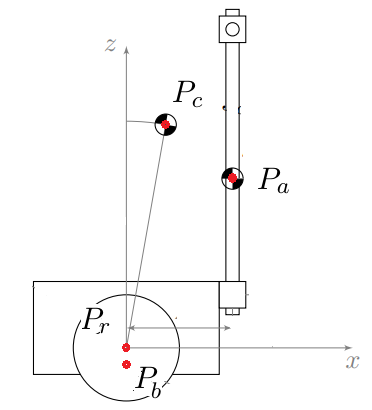
\includegraphics[width=0.4\textwidth]{Immagini/VAB_baricentrum.png}
	\caption{Baricentri dei singoli corpi rigidi}
	\label{fig:VAB_baricentri}
\end{figure} 

\subsection{Grandezze di supporto}
Prima di andare a definire le componenti di energia potenziale e cinetica di ogni singolo corpo, siamo andati ad introdurre alcune grandezze geometriche di supporto che definiremo qui di seguito.

Nello specifico abbiamo introdotto i seguenti parametri, specificati anche in figura ~\ref{fig:VAB_lunghezze}:
\begin{itemize}
	\item $\mathbf{l_a}$: rappresenta la congiungente tra il centro del sistema di riferimento \textit{XZ} e il centro dell'asta, utilizzata appunto come manubrio, individuato come
	\begin{center}
		{$l_a = \sqrt{(\frac{h_a}{2} + \frac{h_b}{2})^2 + (\frac{w_b}{2})^2}$}
	\end{center}
	\item $\mathbf{l_c}$: questa grandezza rappresenta per noi l'altezza del baricentro del corpo dell'utente, la quale ovviamente andrà a dipendere dal valore di inclinazione del corpo stesso.
	Considerando il corpo inzialmente in posizione verticale, avremo che questa lunghezza corrisponde alla congiungente dal centro del sistema di riferimento al punto $P_c$, che equivale a dire:
	\begin{center}
		$l_c = 0.55 h_c + \frac{h_b}{2}$
	\end{center}
	\item $\mathbf{l_b}$: rappresenta lo spostamento verso il basso, lungo l'asse z, del baricentro dello chassis. Da specifiche del progetto sappiamo che questa grandezza ha valore (con segno negativo) di
	\begin{center}
		$l_b = 0.1 m$
	\end{center}
	\item $\mathbf{\beta}$: angolo formato con la verticale dalla congiungente tra il centro del sistema di riferimento e il punto $P_a$. Si ricava, con un semplice approccio trigonometrico che, l'angolo in questione, ha questa forma:
	\begin{center}
		$\arctan{(\frac{\frac{w_b}{2}}{\frac{h_a}{2} + \frac{h_b}{2}})}$
	\end{center}
\end{itemize}

\begin{figure}[h]
	\centering   	
	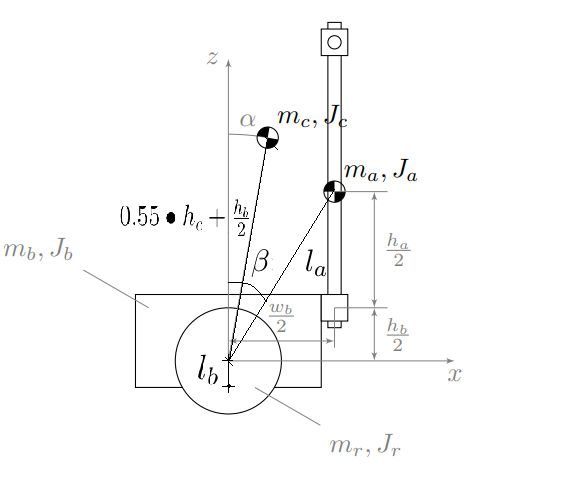
\includegraphics[width=0.6\textwidth]{Immagini/VAB_additionalMeasures.png}
	\caption{Grandezze di supporto}
	\label{fig:VAB_lunghezze}
\end{figure}

\subsection{Calcolo componenti dinamiche e potenziali per ogni corpo rigido del sistema}
Per ognuno dei corpi rigidi definiti in precedenza siamo andati appunto a calcolare:

\begin{itemize}
	\item \textbf{Coordinate spaziali P} espresse nel sistema di riferimento XZ. A queste due coordinate cartesiane ne va aggiunta una terza, relativa alle coordinate angolari (per poter tener così conto dei contirbuti inerziali dei corpi);
	\item \textbf{Vettore delle velocità V} $\rightarrow$ vettore $3\times 1$
	\item \textbf{Matrice delle masse M} $\rightarrow$ matrice $3\times 3$
	\item \textbf{Energia cinetica T} $\rightarrow \frac{1}{2} V^T M V$
	\item \textbf{Energia potenziale U}
	\item \textbf{Lagrangiana \textit{parziale} L del singolo corpo rigido}
\end{itemize}

\subsubsection{Asta}
\begin{itemize}
	
	\item \textbf{$P_a = \left(\begin{array}{c}
		r\,\phi \left(t\right)+l_a \,\mathrm{sin}\left(\beta +\theta \left(t\right)\right)\\
		l_a \,\mathrm{cos}\left(\beta +\theta \left(t\right)\right)\\
		\theta \left(t\right)
		\end{array}\right)$}
	\\\\
	\item \textbf{$V_a = \left(\begin{array}{c}
		r\,\dot{\phi \left(t\right)}+l_a \,\mathrm{cos}\left(\beta +\theta \left(t\right)\right)\,\dot{\theta \left(t\right)}\\
		-l_a \,\mathrm{sin}\left(\beta +\theta \left(t\right)\right)\,\dot{\theta \left(t\right)}\\
		\dot{\theta \left(t\right)}
		\end{array}\right)$}
	\\\\
	\item \textbf{$M_a = \left(\begin{array}{ccc}
		m_a  & 0 & 0\\
		0 & m_a  & 0\\
		0 & 0 & m_a \,{l_a }^2 +J_a 
		\end{array}\right)$}
	\\\\
	\item \textbf{$T_a = m_a \,{l_a }^2 \,{{\left(\dot{\theta \left(t\right)}\right)}}^2 +\frac{m_a \,r^2 \,{{\left(\dot{\phi \left(t\right)}\right)}}^2 }{2}+\frac{J_a \,{{\left(\dot{\theta \left(t\right)}\right)}}^2 }{2}+m_a \,\mathrm{cos}\left(\beta +\theta \left(t\right)\right)\,l_a \,r\,\dot{\theta \left(t\right)}\,\dot{\phi \left(t\right)}$}
	\\
	\item \textbf{$U_a = g\,l_a \,m_a \,\mathrm{cos}\left(\beta +\theta \left(t\right)\right)$}
	\\
	\item \textbf{$L_a = m_a \,{l_a }^2 \,{{\left(\dot{\theta \left(t\right)}\right)}}^2 +\frac{m_a \,r^2 \,{{\left(\dot{\phi \left(t\right)}\right)}}^2 }{2}+\frac{J_a \,{{\left(\dot{\theta \left(t\right)}\right)}}^2 }{2}+m_a \,\mathrm{cos}\left(\beta +\theta \left(t\right)\right)\,l_a \,r\,\dot{\theta \left(t\right)}\,\dot{\phi \left(t\right)}-g\,m_a \,\mathrm{cos}\left(\beta +\theta \left(t\right)\right)\,l_a$}
\end{itemize}
\subsubsection{Chassis (base)}
\begin{itemize}
	
	\item \textbf{$P_b = \left(\begin{array}{c}
		r\,\phi \left(t\right)-l_b \,\mathrm{sin}\left(\theta \left(t\right)\right)\\
		-l_b \,\mathrm{cos}\left(\theta \left(t\right)\right)\\
		\theta \left(t\right)
		\end{array}\right)$}
	\\\\
	\item \textbf{$V_b = \left(\begin{array}{c}
		r\,\dot{\phi \left(t\right)}-l_b \,\mathrm{cos}\left(\theta \left(t\right)\right)\,\dot{\theta \left(t\right)}\\
		l_b \,\mathrm{sin}\left(\theta \left(t\right)\right)\,\dot{\theta \left(t\right)}\\
		\dot{\theta \left(t\right)}
		\end{array}\right)$}
	\\\\
	\item \textbf{$M_b = \left(\begin{array}{ccc}
		m_b  & 0 & 0\\
		0 & m_b  & 0\\
		0 & 0 & m_b \,{l_b }^2 +J_b 
		\end{array}\right)$}
	\\\\
	\item \textbf{$T_b = m_b \,{l_b }^2 \,{{\left(\dot{\theta \left(t\right)}\right)}}^2 +\frac{m_b \,r^2 \,{{\left(\dot{\phi \left(t\right)}\right)}}^2 }{2}+\frac{J_b \,{{\left(\dot{\theta \left(t\right)}\right)}}^2 }{2}-m_b \,\mathrm{cos}\left(\theta \left(t\right)\right)\,l_b \,r\,\dot{\theta \left(t\right)}\,\dot{\phi \left(t\right)}$}
	\\
	\item \textbf{$U_b = -g\,l_b \,m_b \,\mathrm{cos}\left(\theta \left(t\right)\right)$}
	\\
	\item \textbf{$L_b = m_b \,{l_b }^2 \,{{\left(\dot{\theta \left(t\right)}\right)}}^2 +\frac{m_b \,r^2 \,{{\left(\dot{\phi \left(t\right)}\right)}}^2 }{2}+\frac{J_b \,{{\left(\dot{\theta \left(t\right)}\right)}}^2 }{2}-m_b \,\mathrm{cos}\left(\theta \left(t\right)\right)\,l_b \,r\,\dot{\theta \left(t\right)}\,\dot{\phi \left(t\right)}+g\,m_b \,\mathrm{cos}\left(\theta \left(t\right)\right)\,l_b$}
\end{itemize}
\subsubsection{Utente}
\begin{itemize}
	
	\item \textbf{$P_c = \left(\begin{array}{c}
		r\,\phi \left(t\right)+l_c \,\mathrm{sin}\left(\alpha +\theta \left(t\right)\right)\\
		l_c \,\mathrm{cos}\left(\alpha +\theta \left(t\right)\right)\\
		\alpha +\theta \left(t\right)
		\end{array}\right)$}
	\\\\
	\item \textbf{$V_c = \left(\begin{array}{c}
		r\,\dot{\phi \left(t\right)}+l_c \,\mathrm{cos}\left(\alpha +\theta \left(t\right)\right)\,\dot{\theta \left(t\right)}\\
		-l_c \,\mathrm{sin}\left(\alpha +\theta \left(t\right)\right)\,\dot{\theta \left(t\right)}\\
		\dot{\theta \left(t\right)}
		\end{array}\right)$}
	\\\\
	\item \textbf{$M_c = \left(\begin{array}{ccc}
		m_c  & 0 & 0\\
		0 & m_c  & 0\\
		0 & 0 & m_c \,{l_c }^2 +J_c 
		\end{array}\right)$}
	\\\\
	\item \textbf{$T_c = m_c \,{l_c }^2 \,{{\left(\dot{\theta \left(t\right)}\right)}}^2 +\frac{m_c \,r^2 \,{{\left(\dot{\phi \left(t\right)}\right)}}^2 }{2}+\frac{J_c \,{{\left(\dot{\theta \left(t\right)}\right)}}^2 }{2}+m_c \,\mathrm{cos}\left(\alpha +\theta \left(t\right)\right)\,l_c \,r\,\dot{\theta \left(t\right)}\,\dot{\phi \left(t\right)}$}
	\\
	\item \textbf{$U_c = g\,l_c \,m_c \,\mathrm{cos}\left(\alpha +\theta \left(t\right)\right)$}
	\\
	\item \textbf{$L_c = m_c \,{l_c }^2 \,{{\left(\dot{\theta \left(t\right)}\right)}}^2 +\frac{m_c \,r^2 \,{{\left(\dot{\phi \left(t\right)}\right)}}^2 }{2}+\frac{J_c \,{{\left(\dot{\theta \left(t\right)}\right)}}^2 }{2}+m_c \,\mathrm{cos}\left(\alpha +\theta \left(t\right)\right)\,l_c \,r\,\dot{\theta \left(t\right)}\,\dot{\phi \left(t\right)}-g\,m_c \,\mathrm{cos}\left(\alpha +\theta \left(t\right)\right)\,l_c$}
\end{itemize}
\subsubsection{Ruota}
\begin{itemize}
	
	\item \textbf{$P_r = \left(\begin{array}{c}
		r\,\phi \left(t\right)\\
		0\\
		\phi \left(t\right)
		\end{array}\right)$}
	\\\\
	\item \textbf{$V_r = \left(\begin{array}{c}
		r\,\dot{\phi \left(t\right)}\\
		0\\
		\dot{\phi \left(t\right)}
		\end{array}\right)$}
	\\\\
	\item \textbf{$M_r = \left(\begin{array}{ccc}
		m_r  & 0 & 0\\
		0 & m_r  & 0\\
		0 & 0 & J_r 
		\end{array}\right)$} \label{matrix:mr}
	\\\\
	\item \textbf{$T_r = \frac{{\left(m_r \,r^2 +J_r \right)}\,{{\left(\dot{\phi \left(t\right)}\right)}}^2 }{2}$}
	\\
	\item \textbf{$U_r = 0$}
	\\
	\item \textbf{$L_r = \frac{{\left(m_r \,r^2 +J_r \right)}\,{{\left(\dot{\phi \left(t\right)}\right)}}^2 }{2}$}
\end{itemize}

\subsubsection{Veicolo completo}
Una volta trovati le componenti dinamiche dei singoli corpi rigidi, possiamo andare a definire l'energia cinetica e potenziale totale del sistema, per poter poi calcolare l'equazione di Lagrange per l'intero sistema.
In sostanza quindi avremo:
\begin{center}
	$L = L_a + L_b + L_c + 2 L_r$
\end{center}
Quello che ne deriva è quindi la seguente equazione Lagrangiana, in grado di descrivere la dinamica dell'intero sistema (riportiamo il risultato letterale, ovvero non legato alla sostituzione di alcun valore numerico che descrive il sistema):



\begin{center}
	$L = {\left(m_a \,l_a^2 +m_b \,l_b^2 +m_c \,l_c^2 \, +\frac{J_a}{2}+\frac{J_b}{2}+\frac{J_c}{2}\right)}\,({\dot{\theta \left(t\right)}})^2 +
	{\left(m_r \,r^2 +J_r +\frac{m_a \,r^2}{2}+\frac{m_b \,r^2}{2}+\frac{m_c \,r^2}{2}\right)}\,({\dot{\phi \left(t\right)}})^2 +
	{\left(m_c \,\sigma_4 \,l_c \,r +m_a \,\sigma_3 \,l_a \,r -m_b \, cos\left(\theta \left(t\right)\right)\,l_b \,r\right)}\dot{\theta \left(t\right)}\,\dot{\phi \left(t\right)}+
	g\,m_b \,\mathrm{cos}\left(\theta \left(t\right)\right)\,l_b -g\,m_c \,\sigma_4 \,l_c -g\,m_a \,\sigma_3 \,l_a$
	
	$\sigma_3 =\mathrm{cos}\left(\beta +\theta \left(t\right)\right)
	\sigma_4 =\mathrm{cos}\left(\alpha +\theta \left(t\right)\right)$
\end{center}

\subsubsection{Note sul calcolo delle componenti dinamiche}
\begin{itemize}
	\item Nel calcolo della matrice di massa abbiamo considerato tre componenti:
	\begin{itemize}
		\item Componente di massa lungo x;
		\item Componente di massa lungo z;
		\item Componente di massa rotazionale: dalla meccanica è noto che un corpo, con una certa massa che si trova in uno stato di rotazione, avrà un contirbuto inerziale che dipende dal braccio rispetto all'asse intorno al quale avviene la rotazione.
		
		Nello specifico abbiamo considerato il teorema di \textit{Huygens-Steiner} per ogni singolo corpo rigido che è stato preso in esame.
		
		\begin{center}
			$ I_a = I_{cm} + md^2 $	
		\end{center}
		
		Esso permette di definire l'inerzia di un corpo come la somma di due diverse componenti:
		\begin{itemize}
			\item Momento d'inerzia definito rispetto all'asse passante per il centro di massa: questo parametro rappresenta il valore che è fornito dalle specifiche del progetto per gli specifici corpi;
			\item Prodotto tra la massa \textit{m} del corpo preso in considerazione e la distanza tra l'asse rispetto a cui si riferisce la rotazione e quello passante per il centro di massa;
		\end{itemize}
	
		Questa componente inerziale è visibile nelle matrici di massa in posizione $(3, 1)$: si sottolinea come invece, per la matrice di massa relativa alle ruote (matrice $M_r$ ~\ref{matrix:mr}), non sia presente la componente esplicitata dal teorema di \textit{Huygens-Steiner} per il fatto che il centro di massa della ruota coincide con quello del sistema di riferimento XZ e quindi di conseguenza non è necessaria alcuna traslazione di asse;
 	\end{itemize}
 	\item Nel calcolo simbolico in ambiente \textit{Matlab} siamo andati ad utilizzare le funzionalità di \textit{collect} e \textit{simplify}, per permettere di ridurre e semplificare le equazioni. Nello specifico, con il comando simplify, tramite l'opzione \textit{Steps}, siamo andati a settare il numero di step che l'algoritmo di calcolo simbolico andrà ad eseguire per poter ridurre e semplificare il maggior numero di termini possibili ($\uparrow Steps, \uparrow $\textit{Compattezza eq symb});
 	
 	\item Le ruote, nel calcolo della dinamica completa del VAB, sono state considerate con un contirbuto doppio;
 	
 	\item Nello studio dello chassis (base), abbiamo seguito questo approccio: il baricentro della base stessa sappiamo essere posizionato ad una quota differente rispetto al centro del sistem di coordinate XZ preso come riferimento.
 	Per questo motivo il suo contributo in termini cinetici e potenziali dipende dal valore dell'inclinazione dello chassis, ovvero dal valore dell'angolo \textit{caratterizzante} il sistema $\theta$: questo concetto è evidenziato in figura ~\ref{fig:chassis}.
 	L'aggiunta di \textit{$\pi$} al valore di $\theta$ è necessaria per poter rendere sensibile i valori di energia cinetica e potenziale al \textit{quadrante} in cui si trova ad essere posizionato il centro di massa della base stessa ($P_b$).
 	
 	\begin{figure}[h]
 		\centering   	
 		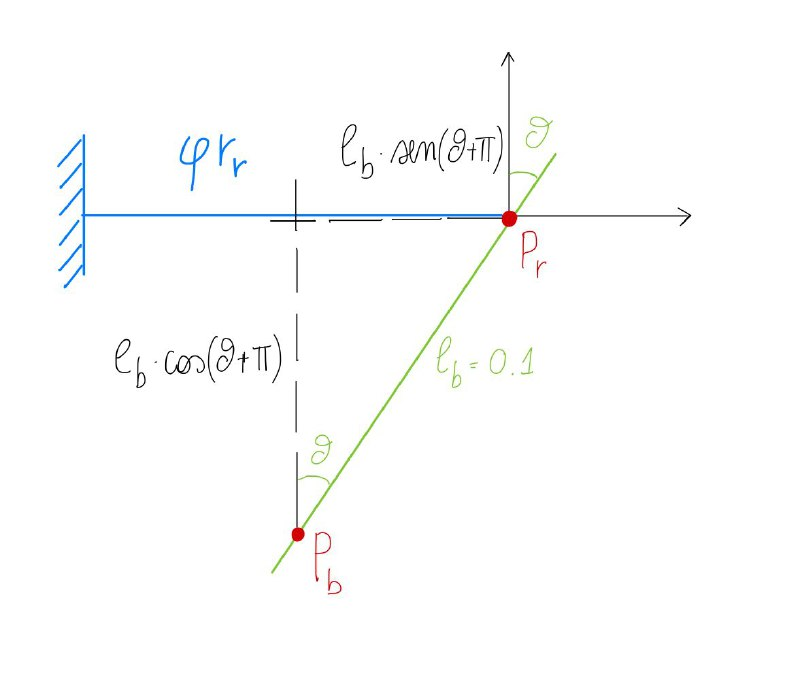
\includegraphics[width=0.6\textwidth]{Immagini/ChassisAngle.jpg}
 		\caption{Ragionamento per il calcolo dei contributi dinamici dello chassis}
 		\label{fig:chassis}
 	\end{figure}
 	
\end{itemize}

\section{Equazioni del moto}
\subsection{Lagrangiana}
Una volta definita la dinamica del sistema ed ottenuta quindi l'equazione di Lagrange che ne caratterizza il comportamento, andiamo a ricavare le equazioni del moto, le quali consentono di definire l'andamento delle \textit{coordinate libere} (scelte in fase inziale di progetto) che sappiamo essere
\begin{itemize}
	\item $\phi = q_1 =$ \textit{angolo di rotazione delle ruote}
	\item $\theta = q_2 =$ \textit{angolo di inclinazione dello chassis}
\end{itemize}

In particolare possiamo definire le cosidette \textit{equazioni di Eulero-Lagrange}, ovvero un insieme di n equazioni differenziali (con n pari al numero di coordinate libere del sistema), la cui risoluzione fornisce le equazioni del moto del sistema.
\begin{center}
	\label{eq:lagrangiana}
	$\frac{d}{\mathrm{dt}}\left(\frac{\partial }{\partial \dot{q_i} }L\right)-\frac{\partial }{\partial q_i}L=\mathrm{Q_i}\ \rightarrow i = 1,...,n$
\end{center}

Sono da effettuare alcune annotazioni sugli addenti presenti nell'equazione precedente  (eq~\ref{eq:lagrangiana}):
\begin{itemize}
	\item \textit{q} rappresenta la coordinata libera (nel nostro caso saranno $\theta$ e $\phi$);
	\item al secondo membro della lagrangiana troviamo le componenti generalizzate, relative alle forze attive esterne. Nel nostro sistema andiamo a modellizzare, come forze attive, quelle che sono le forze motrici immesse dai motori che gestiscono il movimento del V.A.B.: in particolare, nel nostro caso, per il legame matematico tra le componenti generalizzate e il concetto di lavoro virtuale, avremo che l'equazione lagrangiana sarà equiparata al valore di torque immessa dal motore nel sistema;
	\item molto importante, ai fini della correttezza delle equazioni del moto, è il valore da assegnare al secondo membro \textit{torque}; infatti esso varia a seconda che il sistema agisca sulla coordinata libera \textit{q} a valle o a monte della trasmissione.
	
	Nello specifico, si osserva che il motore è composto da due parti: lo statore e il rotore. Esse trasmettono una coppia uguale e inversa ai corpi a cui sono solidalmente collegati: lo statore, posizionato nella base del Segway, influenza la coordinata libera $\theta$ ed esercita una coppia sullo chassis pari ad una generica coppia \textit{$-2 C_m$}.
	Il fattore moltiplicativo 2 è dovuto al fatto che nella base sono presenti due motori.
	
	Nello stesso modo, il rotore, trasmette all'albero motore una coppia \textit{$C_m$}: a valle della trasmissione si misura dunque una coppia \textit{$\frac{C_m}{\tau}$} dovuta alla presenza della trasmissione
	Questa coppia ridotta all'albero dell'utilizzatore è la coppia che in definitiva va ad agire sulle ruote e quindi sulla coordinata $\phi$.
\end{itemize}

\newpage
Si ottiene dunque il seguente sistema di equazioni, la cui risoluzione permette di ottenere due equazioni differenziali del secondo ordine nelle variabili $\theta$ e $\phi$:
\begin{center}
	$
	\begin{cases}
		\label{eq:lagrangiana_theta_phi}
		\begin{array}{c}
			\frac{d}{\mathrm{dt}}\left(\frac{\partial }{\partial \dot{\theta} }L\right)-\frac{\partial }{\partial \theta}L=\mathrm{-2 C_m} \\
			\frac{d}{\mathrm{dt}}\left(\frac{\partial }{\partial \dot{\phi} }L\right)-\frac{\partial }{\partial \phi}L=\mathrm{\frac{C_m}{\tau}}
		\end{array}
	\end{cases}
	$
\end{center}
dove $\tau$ è il rapporto di trasmissione il cui calcolo è riportato nella sezione ~\ref{sec:rapp_di_trasmissione}.
La soluzione di questo sistema di equazioni verrà ad essere utilizzata per rappresentare il comportamento del sistema reale, basandosi su una coppia di equazioni non lineare: questa tematica verrà poi approfondita direttamente nella sezione ~\ref{sec:simulazione_reale}.

\subsection{Rapporto di trasmissione}
\label{sec:rapp_di_trasmissione}
Come da specifiche del progetto, ognuno dei due motori è collegato alle ruote mediante una doppia sequenza di riduttori:
\begin{itemize}
	\item Un primo riduttore epicicloidale con rapporto di trasmissione $\tau_1 = 0.1$;
	\item Un secondo riduttore, una cinghia dentata che presenta un rapporto di trasmissione facilmente calcolabile come rapporto tra il numero dei denti dei due alberi, essendo il passo uguale in entrambi gli alberi.
	\begin{center}
		$\tau_2 = \frac{Numero\_denti\_puleggia\_ingresso}{Numero\_denti\_puleggia\_uscita} = \frac{Z_{in}}{Z_{out}} = \frac{22}{26}$
	\end{center}
\end{itemize}

Il rapporto di trasmissione completo $\tau$ è quindi definito come:
\begin{center}
	$\tau = \tau_1 \cdot{\tau_2} = 0.085$	
\end{center}

\subsection{Sistema non lineare}
La risoluzione del sistema di equazioni sopra riportato permette di ottenere due equazioni differenziali del secondo ordine: queste soluzioni sono state ottenute sfruttando la potnezialità del calcolo simbolico messo a disposizione da Matlab, come si vede nel listato seguente.

\begin{lstlisting} [caption={Risoluzione del sistema di equazioni},captionpos=b]
theta2_diff = subs(theta2,{phi,vel,theta,vel_ang,C_m},{q_1 q_1_p q_2 q_2_p u})
phi2_diff = subs(phi2,{phi,vel,theta,vel_ang,C_m},{q_1 q_1_p q_2 q_2_p u })
\end{lstlisting}

Le soluzioni così ottenute rappresentano e governano la dinamica del sistema: esse verranno quindi utilizzate per andare ad analizzare il comportamento del sistema considerato reale, utlizzando il controllore che è stato progettato sul sistema linearizzato.

Un passaggio importante per la simulazione del sistema non lineare, è quello rappresentato dal salvataggio di queste due equazioni in esame: infatti esse sono, per forza di cose, richiamate all'interno della simulazione \textit{Simulink}: per fare ciò abbiamo utilizzato il comando \textit{matlabFunction()}, il quale va a scrivere in una funzione di matlab le due equazioni in esame.

\begin{lstlisting} [caption={Salvataggio in funzioni Matlab},captionpos=b]
matlabFunction(theta2_diff,'File','theta_secondo');
matlabFunction(phi2_diff,'File','phi_secondo');
\end{lstlisting}

Nello specifico queste funzioni avranno come input i valori da cui dipendono le equazioni differenziali e, componendoli algebricamente tra di loro, fornirà come output i valori di $\ddot{\theta}$ e $\ddot{\phi}$.

TODO (mettere le dipendende di theta pp e phi pp)

\subsection{Linearizzazione}
TODO linearizzazione attorno alla massa 70 kg e rileggere paragrafo

Nell'approccio alla modellistica dei sistemi dinamici, uno step molto importante è quello che concerne la linearizzazione del sistema, ovvero il passaggio da un insieme di equazioni non lineari ad un set di equazioni lineari definite nell'intorno di un punto specifico dello stato del sistema: questo nuovo sistema di equazioni andrà a definire un sistema lineare in grado di approssimare il comportamento dinamico del sistema non lineare vicino all'equilibrio.

Il punto in questione è quello in cui la variazione dello stato del sistema è nullo: deto quindi $\mathbf{x}(t)$ il vettore di stato, l'equilibrio sarà dato da $\dot{\mathbf{x}(t)}$.

Perciò, il passo successivo alla risoluzione del sistema di equazioni di Lagrange in $\theta$ e $\phi$ che è stato svolto riguarda la linearizzazione: nel contesto del controllo, linearizzare è importante poiché permette di progettare il controllore stesso sul sistema tangente a quello reale (ovvero il sistema lineare), potendo poi testarlo direttamente sul sistema reale (ovvero quello descritto da equazioni non lineari).

\subsubsection{Calcolo della posizione di equilibrio}
Per poter quindi procedere con la linearizzazione, è necessario innanzitutto calcolare l'equilibrio del sistema, cioè il punto in cui $\mathbf{\ddot{\theta} = 0}$: questa condizione corrisponde  ad una situazione in cui lo stato del sistema risulta essere in una condizione di equilibrio dinamico, ovvero quando la sua variazione nel tempo è nulla (nessuna accelerazione $\rightarrow$ velocità costante $\rightarrow$ posizione lineare):
\begin{center}
	$\left(\begin{array}{c}
		-0.01174364-\text{7.105427e-15}\,\mathrm{i}\\
		3.129849-\text{7.105427e-15}\,\mathrm{i}
	\end{array}\right)$
\end{center}

Queste posizioni di equilibrio le abbiamo ottenute per mezzo della istruzione Matlab ~\ref{code:matalab_eq}, nella quale si vede come, partendo dall'equazione differenziale del sistema non lineare espressa in termini di $\ddot{\theta}$ si ricava la posizione di equilibrio del sistema.
\begin{lstlisting} [caption={Calcolo posizione di equilbrio},captionpos=b]
equilibri = solve(subs(theta2_differenziabile,{q_1 q_1_p q_2_p u},{0,0,0,0})==0,q_2)
\end{lstlisting}

Come si vede, siamo interessati solamente al valore di equilibrio relativo di $\theta$: per questo motivo che poniamo a 0 (valore arbitrario) i valori di $\phi$ e $\dot{\phi}$, poichè non risultano essere di interesse per il calcolo dell'equilibrio.

I risultati ottenuti sono, con buona approssimazione, considerabili numeri naturali e rispondono a quanto ci aspettavamo: essendo presente un offset ($w_b$) tra quello che è il baricentro del sistema di riferimento e quello relativo al manubrio, non ci aspettavamo di ottenere due equilibri perfettamente di 0° (posizione verticale a "testa in sù") e di 180° (posizione verticale a "testa in giù").

Per completezza e per avere comunque un feedback più concreto, abbiamo provato ad azzerare il valore di $w_b$, andando a ricalcolare la posizione di equilibrio, ottenendo effettivamente i valori di
\begin{center}
	$\left(\begin{array}{c}
	0 \text{ deg}\\
	180 \text{ deg}
	\end{array}\right)$
\end{center}

Dal risultato ottenuto, considerando nulla la componente immaginaria, possiamo notare che (osservazioni comuni per i sistemi assimilabili al pendolo):

\begin{itemize}
	\item il sistema ha due equilibri; il primo ($\theta = -0.01174364 \text{ rad} = -0.67 \text{ deg}$) ci si aspetta che sia instabile in quanto il baricentro del sistema V.A.B. (compreso di utente a bordo) risulta essere sopra all'asse delle ruote;
	\item il secondo ($\theta = 3.129849 \text{ rad} = 179.32 \text{ deg}$) è un equilibrio stabile, poiché il baricentro sta sotto l'asse delle ruote e, un eventuale disturbo dopo un certo tempo di transitorio, risulterebbe avere effetto nullo sullo stato del sistema, che ritornerebbe alla medesima posizione;
\end{itemize}

\subsubsection{Calcolo del sistema lineare}
Ovviamente, ai fini del controllo, si è linearizzato attorno al primo equilibrio; non avrebbe infatti senso controllare il sistema quando questo risulta essere capovolto (cosa che per di più risulta essere fisicamente impossibile, se il veicolo autobilanciato viene fatto muovere su una superficie).

I vettori che definiscono le \textbf{variabili di stato del sistema} e le \textbf{uscite del sistema} sono i seguenti:
\begin{center}
	$
	x=\text{variabili di stato = }\left\lbrack 
	\begin{array}{c}
		x_1 \to \phi\\
		x_2 \to \dot{\phi}\\
		x_3 \to \theta\\
		x_4 \to \dot{\theta} 
	\end{array}\right\rbrack
	$
	
	$
	y=\text{output del sistema = }\left\lbrack 
	\begin{array}{c}
		y_1 \to \ddot{\theta}\\
		y_2 \to \ddot{\phi}
	\end{array}\right\rbrack
	$
\end{center}

Per individuare il risultato finale della linearizzazione, abbiamo seguito un approccio matriciale: nello specifico abbiamo utilizzato la notazione matriciale nel caso di sistemi SIMO (\textit{Single Input Multiple Output}), la cui stesura ha utilizzato le seguenti funzioni di supporto:

\begin{center}
	$
	\begin{cases}
		\begin{array}{c}
			\mathbf{f_1} \to {\dot{x_1} \left(t\right)} =\overline{x_2 } =0\text{ (poichè all'equilibrio)}\\
			\mathbf{f_2} \to {\dot{x_2} \left(t\right)} = {\ddot{\phi} \;}\\
			\mathbf{f_3} \to {\dot{x_3} \left(t\right)} =\overline{x_4 } =0\text{ (poichè all'equilibrio)}\\
			\mathbf{f_4} \to {\dot{x_4} \left(t\right)=} {\ddot{\theta} \;}\\
			\mathbf{g_1} \to y_{1\;} \left(t\right)=\phi = x_{1\;}\\
			\mathbf{g_2} \to y_{2\;} \left(t\right)=\theta =x_{2\;}\\
		\end{array}
	\end{cases}
	$
\end{center}

Sfruttando le caratteristiche \textit{matematiche} del sistema non lineare, ottenibili tramite lo sviluppo in serie di Taylor nell'intorno dell'equilibrio, possiamo definire i termini matriciali che permettono di definire il sistema, secondo le seguenti equazioni:

\begin{center}
	$$
	\begin{cases}
		\begin{array}{c}
		\dot{x}\left(t\right) = Ax(t) + Bu(t)\\
		y\left(t\right) = Cx(t) + Du(t)\\
		\end{array}
	\end{cases}
	$$
	$
	A=\left\lbrack
	\begin{array}{cccc}
		\frac{\partial }{\partial x_1 }f_{1\;}  & \frac{\partial }{\partial x_2 }f_{1\;}  & \frac{\partial }{\partial x_3 }f_{1\;}  & \frac{\partial }{\partial x_4 }f_{1\;} \\\\
		\frac{\partial }{\partial x_1 }f_{2\;}  & \frac{\partial }{\partial x_2 }f_{2\;}  & \frac{\partial }{\partial x_3 }f_{2\;}  & \frac{\partial }{\partial x_4 }f_{2\;} \\\\
		\frac{\partial }{\partial x_1 }f_3  & \frac{\partial }{\partial x_2 }f_3  & \frac{\partial }{\partial x_3 }f_3  & \frac{\partial }{\partial x_4 }f_3 \\\\
		\frac{\partial }{\partial x_1 }f_4  & \frac{\partial }{\partial x_2 }f_4  & \frac{\partial }{\partial x_3 }f_4  & \frac{\partial }{\partial x_4 }f_4 
	\end{array}\right\rbrack
	$
	$
	B=\left\lbrack 
	\begin{array}{c}
		\frac{\partial }{\partial u}f_1 \\\\
		\frac{\partial }{\partial u}f_2 \\\\
		\frac{\partial }{\partial u}f_3 \\\\
		\frac{\partial }{\partial u}f_4 
	\end{array}\right\rbrack
	$
	$
	C=\left\lbrack 
	\begin{array}{cccc}
		\frac{\partial }{\partial x_1 }g_{1\;}  & \frac{\partial }{\partial x_2 }g_{1\;}  & \frac{\partial }{\partial x_3 }g_{1\;}  & \frac{\partial }{\partial x_4 }g_{1\;} \\\\
		\frac{\partial }{\partial x_1 }g_{1\;}  & \frac{\partial }{\partial x_2 }g_{1\;}  & \frac{\partial }{\partial x_3 }g_{1\;}  & \frac{\partial }{\partial x_4 }g_2 
	\end{array}\right\rbrack
	$
	$$
	\;D=\left\lbrack \begin{array}{cc}
		\frac{\partial }{\partial u}g_{1\;}  & \frac{\partial }{\partial u}g_2 
	\end{array}\right\rbrack
	$$
\end{center}

Nel specifico del veicolo autobilanciato, nel caso con utente con peso di \textit{70 kg} e altezza \textit{1.77 m}, siamo andati ad ottenere i seguenti valori numerici per le matrici in esame:

\begin{center}
	$
	A=\left\lbrack
	\begin{array}{cccc}
		0  & 1.0  & 0  & 0 \\\\
		0 & 0 & -15.2286 & 0 \\\\
		0  & 0  & 0  & 1.0 \\\\
		0  & 0  & 5.43924 & 0
	\end{array}\right\rbrack
	$
	$
	B=\left\lbrack \begin{array}{c}
		0 \\\\
		2.7498 \\\\
		0 \\\\
		-0.2612 
	\end{array}\right\rbrack
	$
	$
	C=\left\lbrack 
	\begin{array}{cccc}
		1  & 0 & 0 & 0 \\\\
		0  & 1 & 0  & 0
	\end{array}\right\rbrack
	$
	$$
	\;D=\left\lbrack 
	\begin{array}{cc}
		0 & 0
	\end{array}\right\rbrack
	$$
\end{center}


Ricordando infine che un generico sistema dinamico può essere scritto come:

\begin{center}
	$
	G\left(s\right)=C {\left(\mathrm{sI}-A\right)}^{-1} B+D
	$
\end{center}
sostituendo i valori numerici matriciali ottenuti al passo precedente, possiamo ottenere il sistema di equazioni, le quali rappresentano l'insieme delle funzioni di trasferimento caratterizzanti il sistema:

\begin{center}
		$$
		\left(\begin{array}{c}
		\frac{2.75}{s^2 }-\frac{\text{1.749e+13}}{\text{2.392e+13}\,s^2 -\text{4.398e+12}\,s^4 }\\ \\
		\frac{2.75}{s}-\frac{\text{1.749e+13}}{\text{2.392e+13}\,s-\text{4.398e+12}\,s^3 }\\ \\
		-\frac{\text{1.149e+12}}{\text{4.398e+12}\,s^2 -\text{2.392e+13}}\\ \\
		-\frac{\text{1.149e+12}\,s}{\text{4.398e+12}\,s^2 -\text{2.392e+13}}
		\end{array}\right)
		$$
\end{center}
Si può notare come la prima e la seconda riga della matrice differiscano solo per un fattore derivativo, così come la terza e quarta riga; questo è ovvio ed atteso in quanto $x_2$ è a derivata di $x_1$ e $x_4$ la derivata di $x_3$.

Nello specifico, queste funzionalità di linearizzazione, sono state racchiuse all'interno del \textit{live script} Matlab nominato \textit{VAB\_simulazioni\_discrete.mlx}: in questo modo siamo stati in grado di rendere più efficace ed efficiente la prosecuzione della simulazione, non dovendo eseguire ogni volta anche questa parte di calcolo matematico relativo alla linearizzazione. Siamo andati infatti a sfruttare le funzionalità di salvataggio offerte da Matlab, per salvare in un file \textit{.mat} l'intera \textit{workspace} (file che abbiamo nominato \textit{WS\_VAB\_wb\_0\_5.mat}), in maniera tale da permettere, agli script che ne avessero bisogno, di aprire il workspace e leggere tutte le variabili di interesse.

	\chapter{Controllo}
	\chapter{OPC - UA}
\chapter{Rumore}
Piattaforma inerziale --> PSD
Questione anti windup --> coppia già limitata quindi nessun vincolo di saturazione
	\chapter{Simulink}
	\chapter{Simulazione}

TODO: rivdere questa introduzione (io la rivedrei)

Data la straordinarietà degli eventi che erano in corso dal punto di vista sanitario nel nostro paese si è reso necessario svolgere gran parte del lavoro in modalità a distanza e quindi senza la possibilità di testare il modello matematico appena ottenuto e i successivi risultati dovuti all'azione di controllo sul V.A.B., il lavoro quindi è stato svolto per la maggior parte sfruttando il tool \textit{Simulink} di Matlab che è, in poche parole, un risolutore di equazioni differenziali.

Abbiamo così adottato una metodologia di lavoro basata su prototipi sempre più simili a quello che dovrebbe essere il sistema reale.

Si va ora ad analizzare la risposta del sistema al controllo ottenuto nei punti precedenti, per assicurarci, che quanto scritto sopra valga oltre che nella teoria anche nella pratica:
\begin{figure}[H]
	\centering   	
	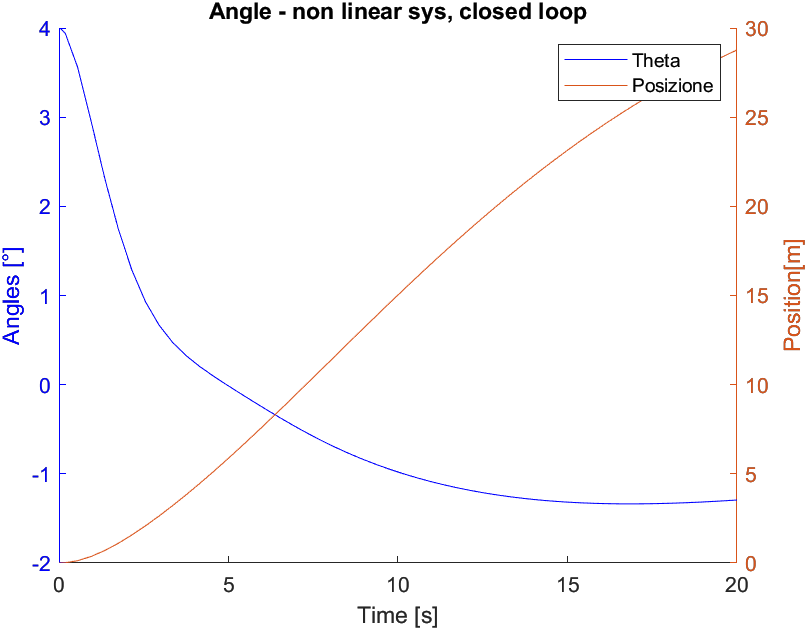
\includegraphics[width=0.7\textwidth]{Immagini/closed_loop_non_linear.png}
	\caption{Risposta del sistema non lineare in anello chiuso}
	\label{fig:closed_loop_non_linear_response}
\end{figure}
\begin{figure}[H]
	\centering   	
	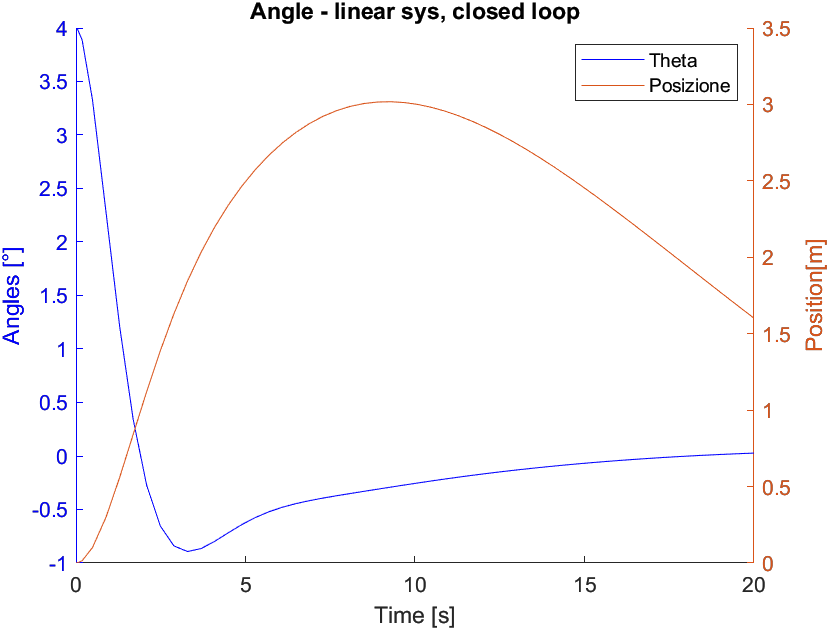
\includegraphics[width=0.7\textwidth]{Immagini/closed_loop_linear.png}
	\caption{Risposta del sistema lineare in anello chiuso}
	\label{fig:closed_loop_non_linear_response}
\end{figure}
TODO: come spieghiamo la differenza? rifare la simulazione?


\section{Simulazione del sistema lineare}

\section{Simulazione del sistema reale}
\label{sec:simulazione_reale}

\section{Discretizzazione}

Il primo compito che abbiamo risolto è stato quello di implementare le equazioni differenziali ottenute nel capitolo precedente:
\begin{itemize}
	\item $\ddot{\phi} = f_{\ddot{\phi}} (M_c,\theta,\dot{\theta},C_m)$
	\item $\ddot{\theta} = f_{\ddot{\theta}} (M_c,\theta,\dot{\theta},C_m)$
\end{itemize}

Dove $M_c$ sarebbe la massa del passeggero, $\theta e \dot{\theta}$ lo stato del sistema e $C_m$  la coppia erogata dal motore. Si può notare come entrambe le equazioni differenziali siano indipendenti dalla coordinata libera $\phi$.
 \begin{figure}[H]
	\centering   	
	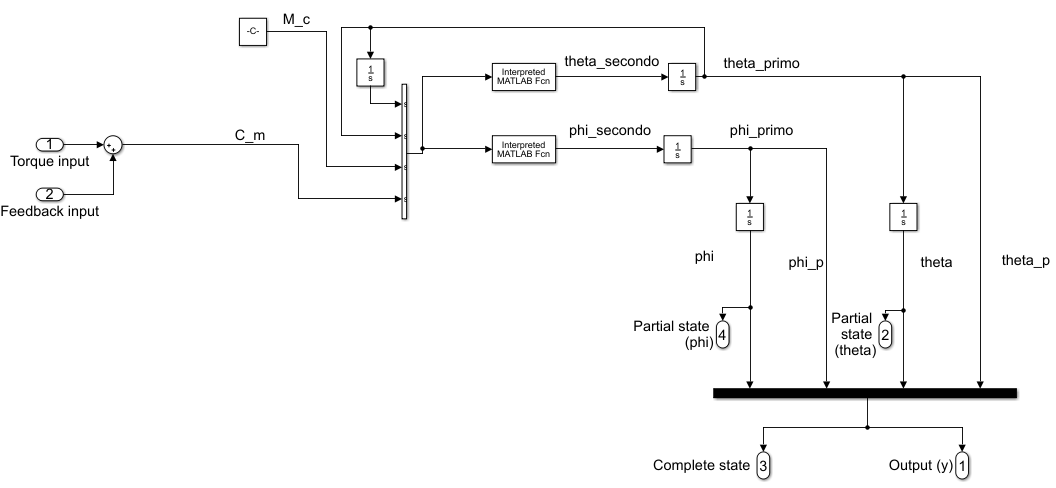
\includegraphics[width=1\textwidth]{Immagini/non_linear_system.png}
	\caption{Implementazione simulink delle equazioni differenziali}
	\label{fig:non_linear_system}
\end{figure}
In Fig.\ref{fig:non_linear_system} le \textit{interpreted function} altro non sono che  $f_{\ddot{\phi}}$ e $f_{\ddot{\theta}}$. A valle di esse sono presenti degli integratori che permettono di ottenere lo stato $x$ completo del sistema. Si può facilmente notare come $\dot{\theta} e \theta$ siano collegate direttamente all'input delle \textit{interpreted function}.
Si è dunque proceduto a  simulare il sistema per verificare la bontà di quanto ottenuto; in particolare, il sistema in anello aperto, dovrebbe oscillare all'infinito vista la mancanza di attriti nel modello.

\begin{figure}[H]
	\centering   	
	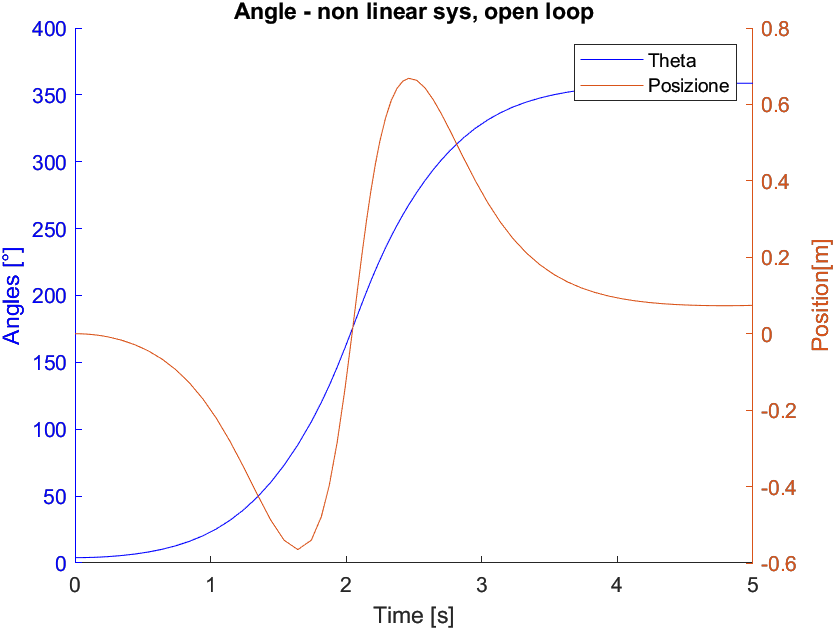
\includegraphics[width=0.6\textwidth]{Immagini/open_loop_response_non_linear.png}
	\caption{Risposta in anello aperto del sistema reale}
	\label{fig:open_loop_response_non_linear}
\end{figure}
La simulazione, il cui risultato è riportato in Fig.\ref{fig:open_loop_response_non_linear} è stata svolta per 5 secondi e con un angolo iniziale di 4°; il grafico mostra dunque l'andamento di $\theta$ nel tempo e della posizione che in termini matematici si esprime come $posizione = \phi \cdot{r_{ruota}}$
Si è inoltre creato un altro modello sfruttando il sistema lineare ottenuto prima  con l'obbiettivo di semplificare il problema e di velocizzare le simulazioni con lo scopo di testare rapidamente nuove tecniche di controllo che se avessero dato esito positivo sul modello lineare sarebbero poi state testate sul simulink che imita il comportamento reale del sistema.
\begin{figure}[H]
	\centering   	
	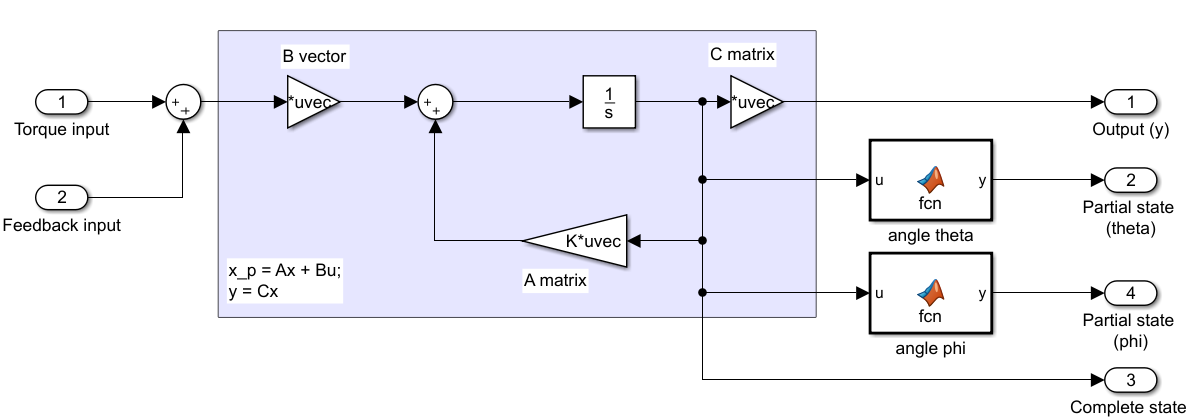
\includegraphics[width=1\textwidth]{Immagini/linear_system.png}
	\caption{Implementazione simulink del sistema linearizzato}
	\label{fig:linear_system}
\end{figure}

\begin{figure}[H]
	\centering   	
	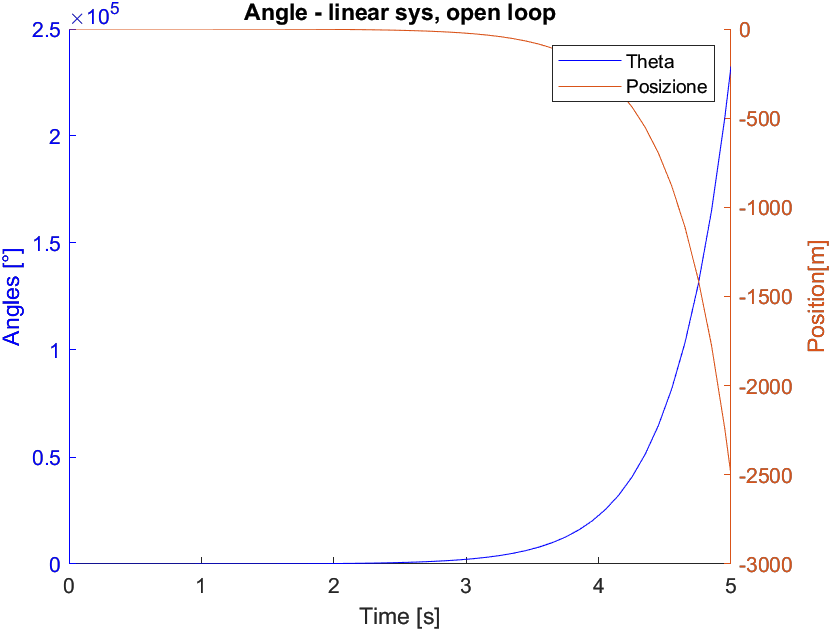
\includegraphics[width=0.6\textwidth]{Immagini/linear_open_loop.png}
	\caption{Risposta in anello aperto del sistema lineare}
	\label{fig:open_loop_response}
\end{figure}
In questo caso, la simulazione in anello aperto mostra che il sistema diverge; questo perché la linearizzazione ha senso attorno al punto di equilibrio da cui è stata ottenuta, distante da quel punto il sistema lineare non approssima più il sistema reale ed anche un eventuale controllo ottenuto da esso non garantisce buone performance distante da quel punto. Si nota, in Fig.\ref{fig:open_loop_response} che il punto di partenza è 4° e il sistema, lineare, diverga quasi immediatamente; la differenza con la risposta del sistema non lineare in Fig.\ref{fig:open_loop_response_non_linear}
\begin{figure}[H]
	\centering   	
	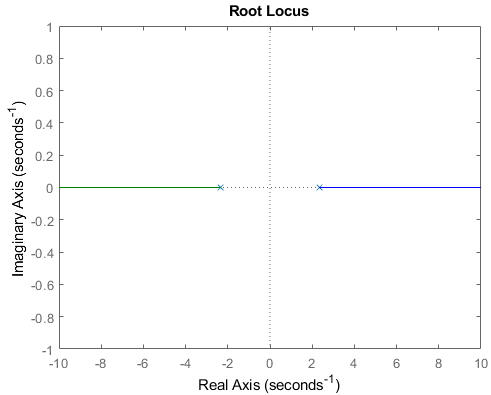
\includegraphics[width=0.6\textwidth]{Immagini/root_locus_open_loop.png}
	\caption{Posizione poli in anello aperto}
	\label{fig:open_loop_root}
\end{figure}
Come si vede in Fig.\ref{fig:open_loop_root}, ci sono due poli reali, uno negativo e uno positivo; questo dimostra come il sistema sia instabile in anello aperto e necessiti di controllo.


\section{Motore}
Il passo successivo è stato quello di andare a modellizzare il motore presente a bordo dello Chassy; questo è necessario in quanto si deve tenere conto, in primo luogo, del ritardo che gli attuatori ( cioè il motore) introducono nel sistema e che per questo potrebbe diventare instabile.
\begin{figure}[H]
	\centering   	
	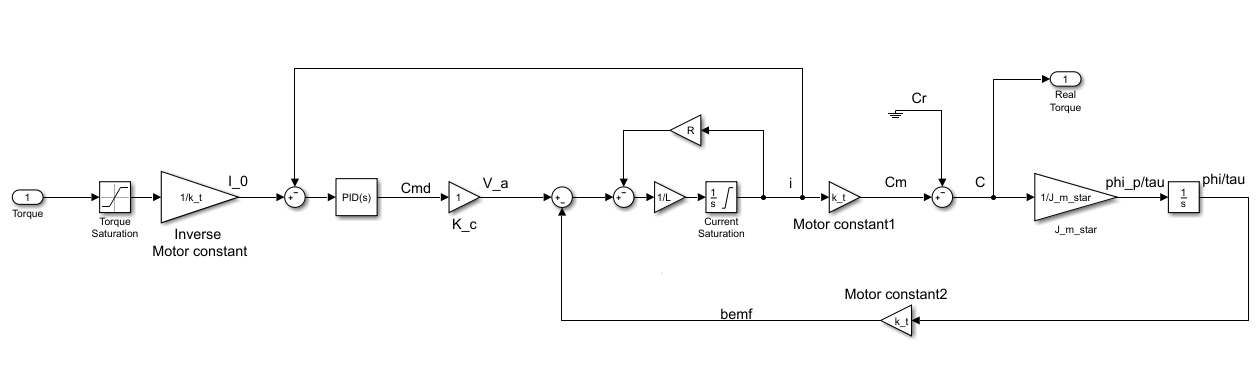
\includegraphics[width=1\textwidth]{Immagini/motor.png}
	\caption{Schema a blocchi del motore}
	\label{fig:motor}
\end{figure}

I valori delle componenti in Fig.\ref{fig:motor} sono presi dal datasheet del motore.
Il controllo del motore DC in questione e stato ottenuto tramite una retroazione in corrente che permette quindi di definire un setpoint alla corrente presente nel motore. Questo si è reso necessario poiché il controllore, attraverso il vettore K e lo stato del sistema, definisce la coppia che il motore dovrebbe erogare. In un motore DC la correlazione tra coppia erogata e corrente esiste ed è ben definita e si tratta di $k_t$.
Il controllore è stato realizzato seguendo metodi già noti in letteratura TODO: scrivere la formula o trovare un posto che la spieghi 
\begin{figure}[H]
	\centering   	
	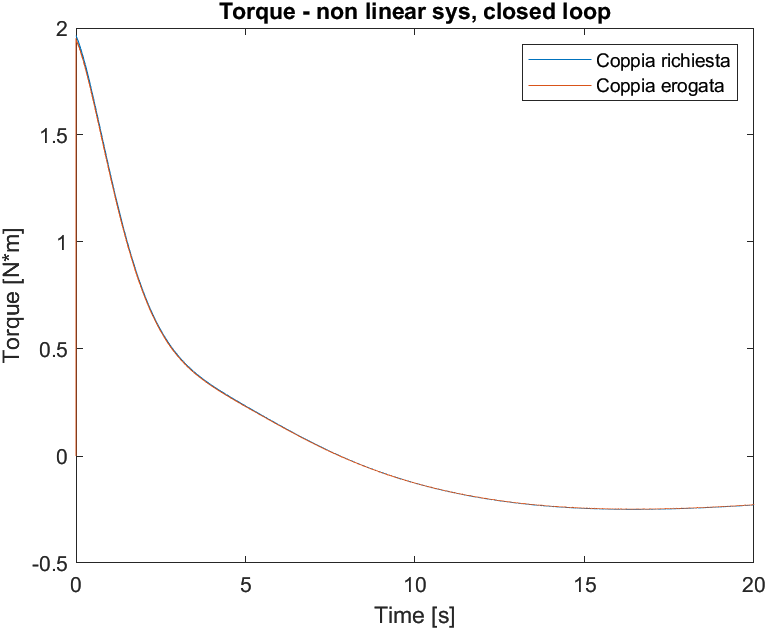
\includegraphics[width=0.7\textwidth]{Immagini/motore.png}
	\caption{Transitorio del motore}
	\label{fig:motore}
\end{figure}
\begin{figure}[H]
	\centering   	
	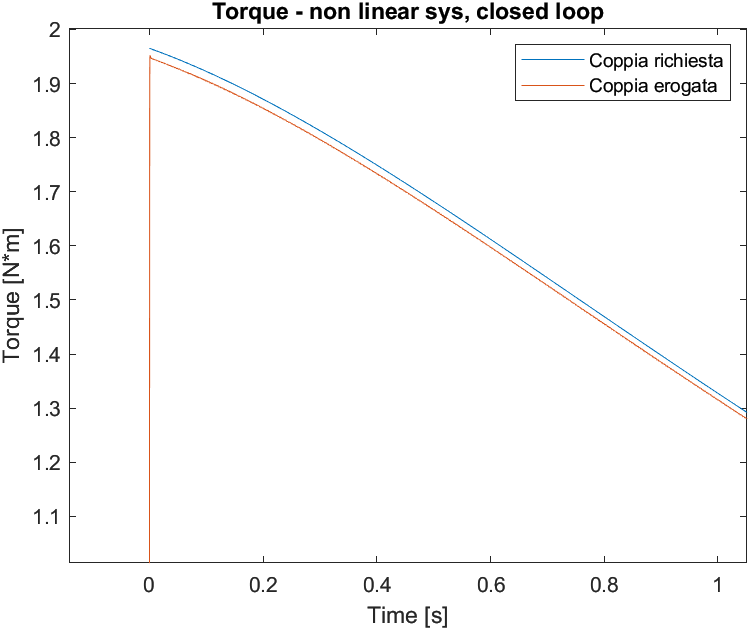
\includegraphics[width=0.7\textwidth]{Immagini/motore_zoom.png}
	\caption{Zoom del grafico in figura Fig.\ref{fig:motore}}
	\label{fig:motore_zoom}
\end{figure}

Come si può notare il picco di coppia massimo è minore di 2; questo è dovuto al fatto che, per ragioni esterne, nel motore può scorrere ua corrente di massimo 20A e quindi:
\begin{center}
	$C_{m,max} = I_{max}\cdot{K_{motore}} = 20 A\cdot{10 \dfrac{N\cdot{m}}{A}}=2N\cdot{m}$
\end{center}

Un esempio in cui la coppia richiesta supera i $2N\cdot{m}$ è il seguente:
\begin{figure}[H]
	\centering   	
	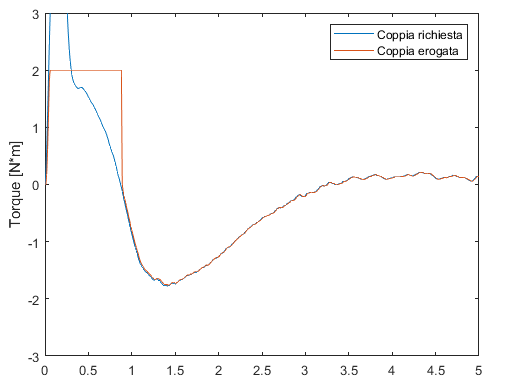
\includegraphics[width=0.8\textwidth]{Immagini/saturazione.png}
	\caption{Clamp della coppia erogata da parte del motore}
	\label{fig:clamp_motore}
\end{figure}
In Fig.\ref{fig:clamp_motore} è anche possibile notare come l'assenza del blocchetto denominato \textit{Torque saturation}, presente in Fig.\ref{fig:motor}, satura l'azione integrale dell'attuatore e inserisce un ritardo non secondario nell'azione di controllo.

	
	\begin{thebibliography}{9}
		\bibitem{feedback_state}
		\emph{Controllo tramite retroazione dello stato,Controlli automatici, Fabio Previdi}
		\url{https://cal.unibg.it/wp-content/uploads/controlli_automatici/Lez06.pdf}
		%%%%%%%%%%%%%%%%%%%%%%%%%%%%%%%%%%%%%%%%%%%%%%%%
	\end{thebibliography}

\end{document}
